\documentclass{article}

% if you need to pass options to natbib, use, e.g.:
% \PassOptionsToPackage{numbers, compress}{natbib}
% before loading nips_2017
%
% to avoid loading the natbib package, add option nonatbib:
% \usepackage[nonatbib]{nips_2017}

\usepackage[final]{nips_2017}

% to compile a camera-ready version, add the [final] option, e.g.:
% \usepackage[final]{nips_2017}

\usepackage[utf8]{inputenc} % allow utf-8 input
\usepackage[T1]{fontenc}    % use 8-bit T1 fonts
\usepackage{hyperref}       % hyperlinks
\usepackage{url}            % simple URL typesetting
\usepackage{booktabs}       % professional-quality tables
\usepackage{amsfonts}       % blackboard math symbols
\usepackage{nicefrac}       % compact symbols for 1/2, etc.
\usepackage{microtype}      % microtypography
\usepackage{amsmath,amsfonts,graphicx,amsthm,amssymb,thmtools}
\usepackage{hyperref}
\usepackage[ruled,vlined]{algorithm2e}
\usepackage{cancel}
\usepackage{multicol}
\usepackage{float}
\usepackage{subcaption}
\usepackage{verbatim}

\newcommand{\indep}{\rotatebox[origin=c]{90}{$\models$}}
\newcommand{\fig}[3]{
			\vspace{#2}
			\begin{center}
			Figure \thelecnum.#1:~#3
			\end{center}
	}
% Use these for theorems, lemmas, proofs, etc.
\theoremstyle{definition}
\newtheorem{theorem}{Theorem}
\newtheorem{example}[theorem]{Example}
\newtheorem{lemma}[theorem]{Lemma}
\newtheorem{proposition}[theorem]{Proposition}
\newtheorem{claim}[theorem]{Claim}
\newtheorem{corollary}[theorem]{Corollary}
\newtheorem{note}[theorem]{Note}
\newtheorem{definition}[theorem]{Definition}
% \newtheorem{problem}{Problem}

% **** IF YOU WANT TO DEFINE ADDITIONAL MACROS FOR YOURSELF, PUT THEM HERE:

\declaretheoremstyle[%
headpunct={\medskip}, postheadspace=\newline, notebraces = {\quad}{},spaceabove = 8pt,spacebelow = 8pt]%
{problem}
\declaretheorem[name=Problem,style=problem]{problem}
\newcommand{\norm}[2]{\left\lVert #1 \right\rVert_{#2}}
\raggedbottom

\title{Improving Robust Manifold Defense}

% The \author macro works with any number of authors. There are two
% commands used to separate the names and addresses of multiple
% authors: \And and \AND.
%
% Using \And between authors leaves it to LaTeX to determine where to
% break the lines. Using \AND forces a line break at that point. So,
% if LaTeX puts 3 of 4 authors names on the first line, and the last
% on the second line, try using \AND instead of \And before the third
% author name.

\author{
  Kwon Jeongyeol \\\texttt{kwonchungli@utexas.edu} \\ University of Texas \And
  Dany Haddad \\\texttt{danyhaddad43@gmail.com} \\ University of Texas
  \And
  Justin Lewis \\\texttt{justin94lewis@utexas.edu} \\
  University of Texas \\
  %% examples of more authors
  %% \And
  %% Coauthor \\
  %% Affiliation \\
  %% Address \\
  %% \texttt{email} \\
  %% \AND
  %% Coauthor \\
  %% Affiliation \\
  %% Address \\
  %% \texttt{email} \\
  %% \And
  %% Coauthor \\
  %% Affiliation \\
  %% Address \\
  %% \texttt{email} \\
  %% \And
  %% Coauthor \\
  %% Affiliation \\
  %% Address \\
  %% \texttt{email} \\
}

\begin{document}
% \nipsfinalcopy is no longer used

\maketitle

\begin{abstract}
  The success of adversarial attacks has brought increased scrutiny
  regarding the robustness of neural networks. A variety of defense
  methods have been proposed, and some of the more promising
  techniques are closely related to the Invert and Classify (INC)
  approach \cite{ilyas2017}. These generative-model based techniques have shown
  hopeful performance in defending a classifier against adversarial examples
  \cite{athalye2018}. The main concern with these methods is their larger drop
  in classification accuracy when compared to other strategies. Here, we propose
  a method that improves the classification accuracy while maintaining
  strong robustness to adversarial examples. Additionally, we present
  preliminary results on MNIST and Fashion-MNIST datasets.
\end{abstract}

\section{Introduction}
 As the vulnerability of classifiers to adversarial examples has gained increasing attention \cite{2014arXiv1412.6572G}, various defense mechanisms have been proposed to robustify classification systems. One such defense, Invert-and-Classify (INC) \cite{ilyas2017}, uses a well-trained generative model to project a potentially adversarial image onto the manifold of natural images. This sister-image can now be safely classified as it no longer contains adversarial components. Additionally, this process is not directly differentiable and therefore seemingly difficult to attack.

% Welcome any correction
In related work, an attack on the INC defense presented by \cite{athalye2018} computed an approximation to the gradient of the entire system by unfolding the optimization process \cite{athalye2018}. However, their survey on attacks against the INC defense was not complete. In particular, they didn't perform an $\ell_{\infty}$ norm attack which is a more common way of attacking a classifier (they only perform an $\ell_2$ attack). Inspired by their idea, we focused on breaking the INC defense by training an encoder that matches the generator used for the defense. We hoped that, together, the generator and encoder form an auto-encoder framework which is directly differentiable and susceptible to adversarial attack. 

Contrary to our intuition, adversarial examples created by connecting a matched encoder were not very useful to break the INC defense. This inadequacy was attributed to our practically imperfect encoder which could not exactly match the INC projection step. This unsuccessful attack empirically convinced us of the non-differentiability of the INC projection, thus mildly confirming the system as robust to any gradient based attacks.

After further experimentation, we discovered that the matched encoder can be used to improve the overall performance of the INC defense. We found empirically that the projection step of the INC system often suffers from bad local optima and thus results in unstable reconstruction. However, the matched encoder we trained gives a good reference point for projection, which in turn not only prevents it from falling into bad local minima, but also expedites the projection. We improved 9\% of the classification accuracy on F-MNIST data where improvement mostly came from good reconstruction. 




\subsection{Contributions}
Our contributions can be summarized as follows (listed in order of importance):
\begin{itemize}
    \item We introduce and formulate the training of a matched encoder to improve the INC defense.
    \item We critique the projection method used in the INC defense and give intuition for its instability.
    \item We provide empirical evidence showing improved classification accuracy for our framework.
\end{itemize}

\section{Background}

\subsection{Notation}

Dataset: $\{\mathcal{X},\mathcal{Y}\}$, a set of images $\mathcal{X}$ and corresponding
class labels $\mathcal{Y}$


Classifier: $\mathcal{C}_{\theta}$

GAN: generator $\mathcal{G}_{\phi}$ and discriminator $\mathcal{D}_{\psi}$

Autoencoder: encoder $\mathcal{E}_{\alpha}$ and decoder $D_\beta$

$x$: a natural image

$x_{adv}$: an adversarial image

\iffalse

\begin{multicols}{3}
%Column 1
Classifier: $\mathcal{C}_{\theta}$
\columnbreak
%Column 2
GAN: generator $\mathcal{G}_{\phi}$ and discriminator $\mathcal{D}_{\psi}$
\columnbreak
%Column 3
AE: encoder $\mathcal{E}_{\alpha}$ and decoder $D_\beta$
\end{multicols}


Given dataset $\{\mathcal{X},\mathcal{Y}\}$, a set of images $\mathcal{X}$ and corresponding
class labels $\mathcal{Y}$, a classifier $\mathcal{C}_{\theta}$ is tasked with correctly labeling the
images in a held-out training set.

A Generative Adversarial Network with generator $\mathcal{G}_{\phi}$ and discriminator $\mathcal{D}_{\psi}$,
is tasked with learning the underlying structure of $\mathcal{X}$ in an unsupervised fashion.
\fi

\subsection{Adversarial Attacks and Training}
The notion of adversarial attacks is a phenomenon brought to light in the context of deep learning by Goodfellow et al. \cite{2014arXiv1412.6572G}. Within this work, it is argued that deep learning classifiers are less robust than previously assumed and susceptible to attack from an adversarial user. More specifically, given image $x$ with correct label $y$ (e.g. "cat") one can add a small perturbation $\delta$ to obtain a new image $x_{adv} = x + \delta$ which is now classified to the wrong label $y_{adv}$ (e.g. "airplane"). This adversarial example is crafted by using knowledge of the classifier $\mathcal{C_{\theta}}$ to maximize the difference between the true label $y$ and adversarial label $y_{adv}$. Given an appropriate notion of loss, $L(y_{adv},y;\theta)$, a canonical adversarial attack is then conducted as follows:

\begin{problem}[Finding an adversarial example]
    \begin{equation*}
    \begin{aligned}
    & \underset{\delta}{\text{maximize}}
    & & L(y_{adv}(\delta),y;\theta) \\
    &
    & & y_{adv}(\delta) = \mathcal{C}_{\theta}(x + \delta) \\
    & \text{subject to}
    & & \norm{\delta}{p} \leq \epsilon
    \end{aligned}
    \end{equation*}
\end{problem}

Plainly said, find the adversarial image $x_{adv} = x + \delta$ within an $\epsilon$ sized $\ell_p$ ball around the
original image which fools the classifier the most. Commonly, this optimization problem is approximately solved using
one of two approaches: Fast Gradient Sign Method (FGSM) and projected gradient descent (PGD). It has been empirically
verified that FGSM attacks are less effective at fooling a classifier than PGD approaches \cite{madry}. Note, a suitable
loss function $L(x,y;\theta)$ might be cross-entropy loss for multi-label classification.


\begin{figure}[H]
    \centering
    \begin{tabular}{ccc}
    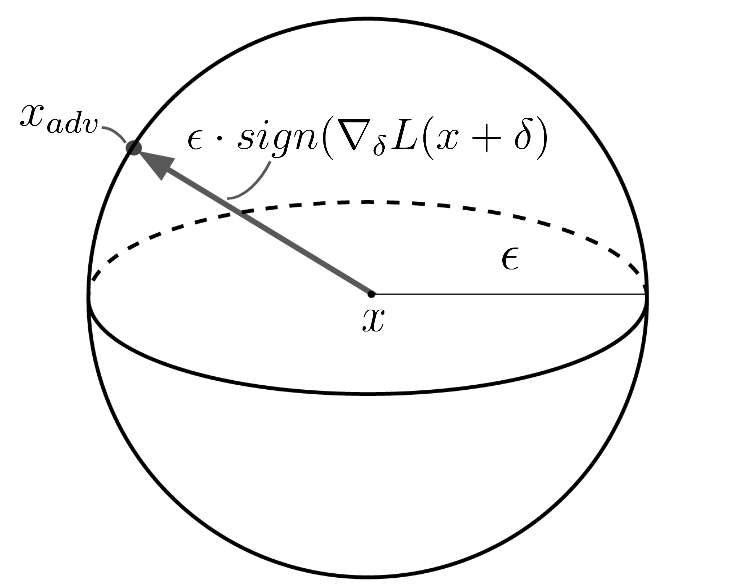
\includegraphics[scale=0.2]{./FGSM.png}
    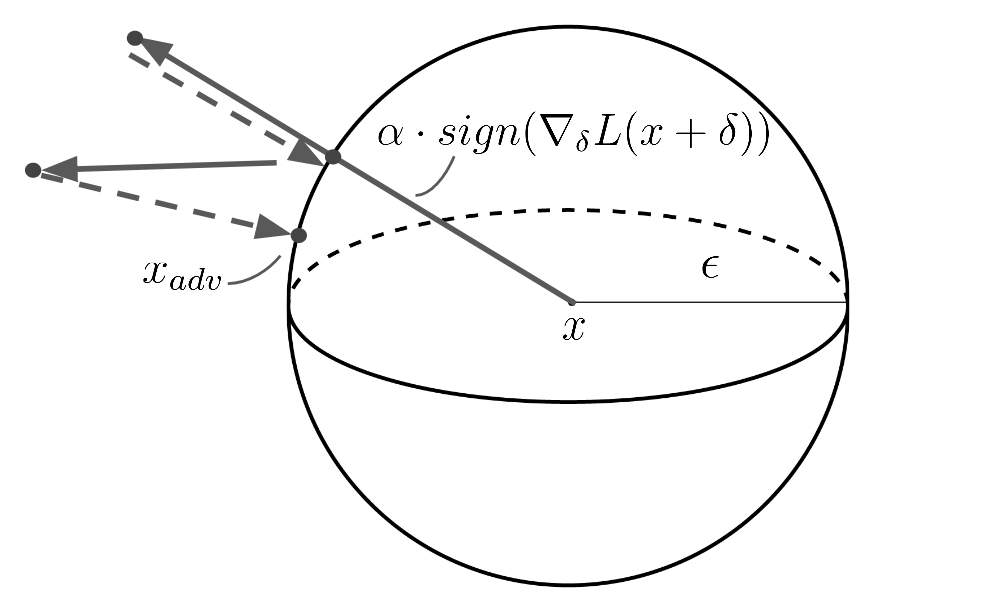
\includegraphics[scale=0.2]{./PGD.png}
    \end{tabular}
    \caption{diagrams demonstrating FGSM (left) and PGD (right) given $\delta$ within an $\ell_2$ ball}
    \label{fig:PGD}
\end{figure}

%There are a number of different environment assumptions that can be made to result in different attack models.
%The above attack is a white-box, non-targeted attack.

In order to defend against adversarial attacks, a number of defense strategies have been employed \cite{athalye2018}.
The most straightforward defense strategies introduce adversarial examples $\mathcal{X}_{adv}$ into the set of training images
$\mathcal{X}$, which allows the network to learn to correctly classify even these examples. Other methods try to
"detect" adversarial examples. These defense strategies give limited robustness guarantees against adversarial examples; moreover, there is large room for improvement regarding defense methods.

\section{Invert and Classify Defense}
The defense strategy of particular interest to our work is the Invert and Classify (INC) approach as introduced by \cite{ilyas2017} and a very similar technique developed by \cite{pixel}. As mentioned before, INC leverages the strong representation power
of GANs. The idea is to project an adversarial image onto the range of a GAN and classify this 'cleaned' image.
This projection is done using gradient descent. If the GAN approximates the manifold of natural images well enough, and
the gradient method projects onto the manifold well enough, then the INC strategy will prove successful.

\begin{figure}[H]
    \centering
    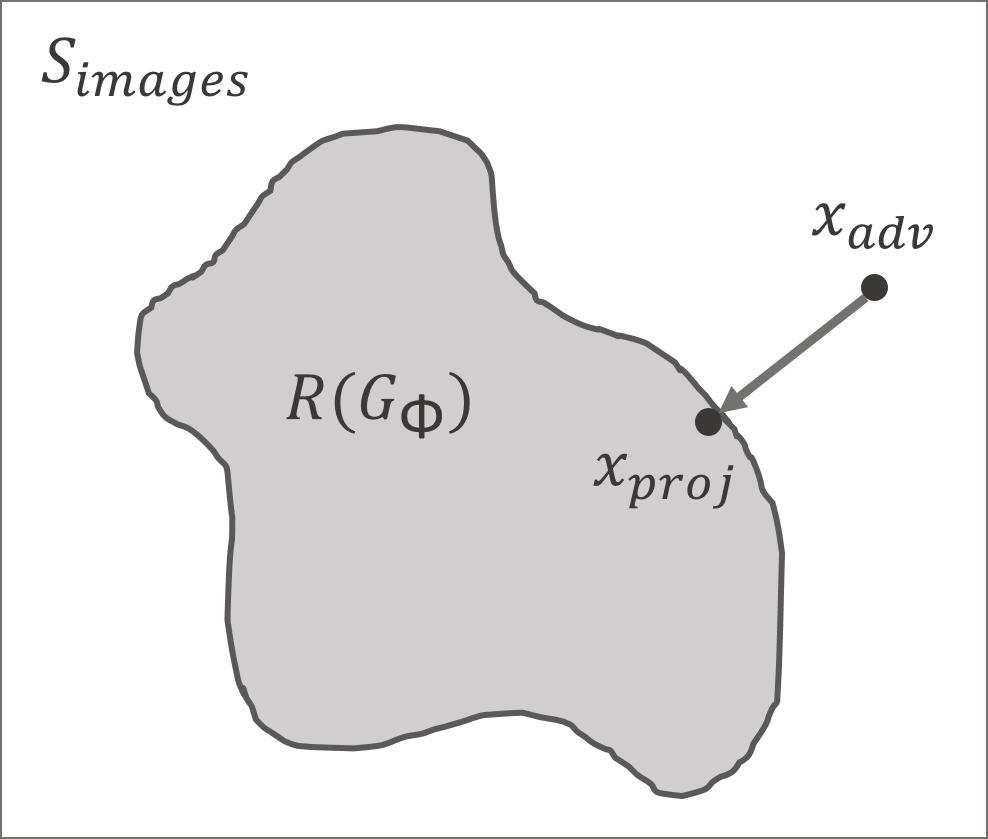
\includegraphics[scale=0.3]{./projection_diagram.png}

    $S_{images}:$ the space of all images

    $R(G_{\phi}):$ the range of the generator
    \caption{abstract diagram demonstrating the inversion portion of INC}
    \label{fig:INC}
\end{figure}

The gradient descent steps search through the latent space $\mathcal{Z}$ for an optimal value $z^*$ which provides the projection $x_{proj} = G_{\phi}(z^*)$. It should be noted that without a trained encoder, the inversion step must begin with a random initialization. It was found empirically in \cite{ilyas2017} that with random initialization, the INC method has poor stability at the output. Therefore, many random initializations were necessary, and the best result was used as the final projection. This repetition of the inversion step is very costly, as it can take hundreds of gradient steps per iteration. The high computation cost of the INC defense is a fairly large drawback. Additionally, even if we perform many random restarts, the final projection might still be far from the optimal point on the feasible set. In section 5 we elaborate on this and provide a solution to this problem. In figure 3 below, the entire INC process is summarized graphically.

\begin{figure}[H]
    \centering
    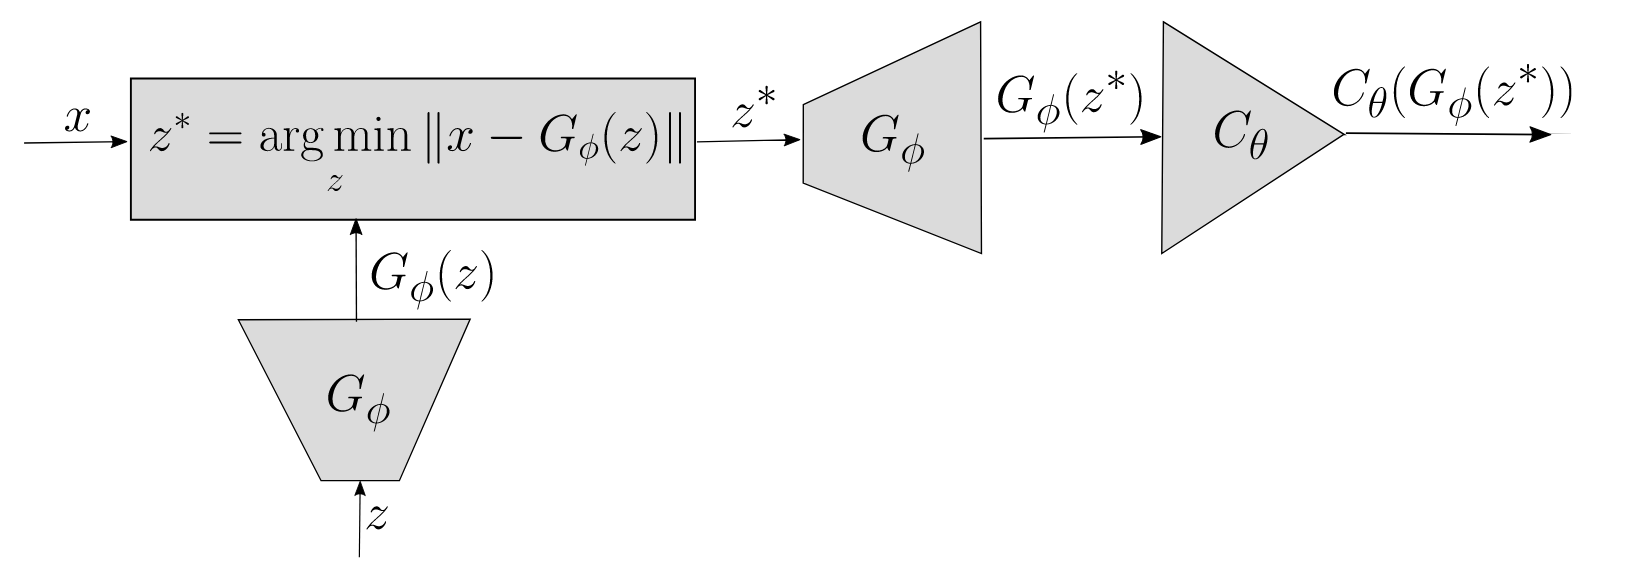
\includegraphics[scale=0.25]{./INC_diagram.png}
    \caption{the INC defense method}
\end{figure}

\begin{problem}[INC projection step (in $\mathcal{Z}$ space)]
    \begin{equation*}
    \begin{aligned}
    & z^* = \text{arg } \underset{z}{\text{min}}
    & & \norm{\mathcal{G}_{\phi}(z)-x_{adv}}{2}^2 \\
    \end{aligned}
    \end{equation*}
\end{problem}

\section{Adversarial Attack on INC}
Similar to the Backward Pass Differentiable Approximation (BPDA) method of Athalye et al., we propose to attack the INC defense mechanism by building a differentiable approximation for the process of projecting onto the manifold of natural images. Using this approximation, we can approximately evaluate the gradient $\nabla_{\delta} L(y_{adv},y) $ and perform gradient based attacks (FGSM and PGD). We learn this approximation by training an encoder  $\mathcal{E}_{\alpha}$ that performs the inverse operation of the generative model used in the INC process. In this way, passing an image through the encoder and pre-trained generator will give us the reconstruction $\hat{x} = \mathcal{G}(\mathcal{E}_{\alpha}(x_{adv}))$. This image serves as an approximation to the result of the INC projection process, $x_{proj}$. To learn this encoder, we approximately solve the following problem by SGD:

\begin{problem}[Learning a matched encoder $\mathcal{E}_{\alpha}$]
    \begin{equation*}
    \begin{aligned}
    & \underset{\alpha}{\text{minimize}}
    & & \mathbb{E}_{Z, \delta} [||\mathcal{E}_{\alpha}(\mathcal{G}(Z) + \delta) - Z||_2^2]
    + \lambda \cdot \mathbb{E}_{X, \delta} [||\mathcal{G}(\mathcal{E}_{\alpha}(X + \delta)) - X||_2^2]\\
    \end{aligned}
    \end{equation*}
\end{problem}

The loss function given in Problem 3 can be interpreted as a sum of two reconstruction loss terms. The first in the latent space $\mathcal{Z}$ and the second in the image space $\mathcal{X}$. Together, the reconstruction terms impose a form of cycle consistency between the image and latent spaces. 

It is important to note that we inject random noise $\delta$ in the image space at each training iteration. By doing so, we ensure the encoder not only learns appropriate reconstruction, but also learns how to project images off the manifold back onto it. In this way, the injected noise $\delta$ acts as a proxy to targeted adversarial noise. 

\begin{figure}[H]
\label{fig:reconstr}
    \caption{matched encoder + generator defence model}
\begin{center}
    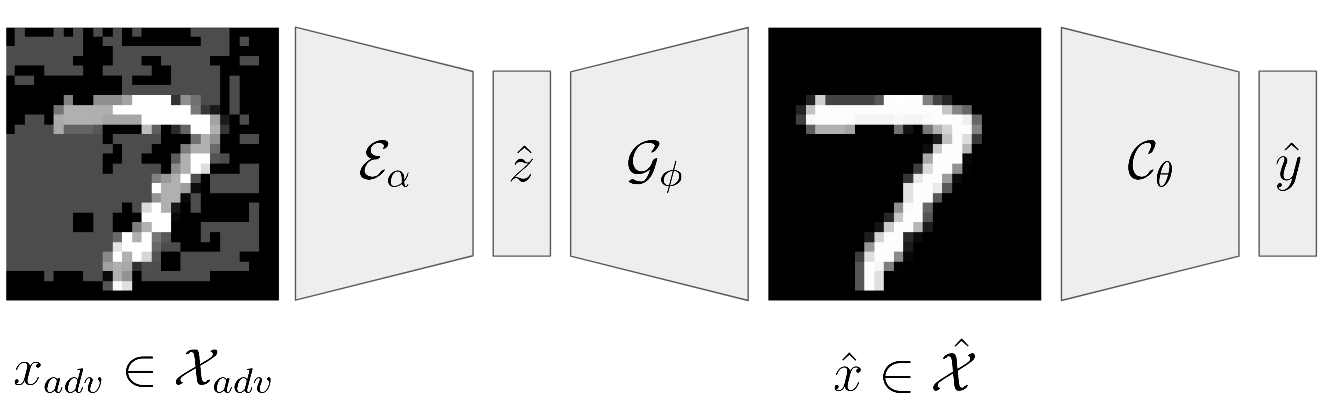
\includegraphics[scale=0.3]{./INC.png}
\end{center}
\end{figure}

We empirically found that training an encoder that perfectly matches the pre-trained generator $\mathcal{G}_{\phi}$ is difficult; however, the reconstruction formed by the composition of encoder and generator was good as shown in fig. \ref{fig:reconstr}.

With a trained encoder $\mathcal{E}_{\alpha}$ and pre-trained generator $\mathcal{G}_{\phi}$ pair, one can now attempt to attack the INC defense by differentiating through the entire classification pipeline. This three-part model is detailed in figure 4. The caveat of our approach is that the trained encoder must sufficiently approximate the projection step from the INC defense, i.e. $\mathcal{E}(x_{adv}) \approx z^*$. To find an adversarial example, we turn to FGSM or PGD to approximately solve the same formulation from Problem 1 with a modified loss which is now parameterized by all three networks. We empirically found that this direct approach was not very effective (the classification accuracy remained at 93\%).

\begin{problem}[Direct adversarial attack on INC]
    \begin{equation*}
    \begin{aligned}
    & \underset{\delta}{\text{maximize}}
    & & L(x+\delta,y;\{\alpha,\phi,\theta\}) \\
    & \text{subject to}
    & & \norm{\delta}{p} \leq \epsilon
    \end{aligned}
    \end{equation*}
\end{problem}

Stepping back, we decided to then attack the INC defense indirectly. With a trained encoder, we could then add adversarial noise to push the encoding $\mathcal{E}(x_{adv})$ as far away from the "true" encoding $\mathcal{E}(x)$ as possible (within the limits of an $\epsilon$ bounded attack).

\begin{problem}[Indirect adversarial attack on INC]
    \begin{equation*}
        \begin{aligned}
        & \underset{\delta}{\text{maximize}}
        & & \norm{\mathcal{E}(x+\delta)-\mathcal{E}(x)}{2}^2 \\
        & \text{subject to}
        & & \norm{\delta}{p} \leq \epsilon
        \end{aligned}
    \end{equation*}
\end{problem}

By pushing the encoding $\mathcal{E}(x_{adv})$ far away, this attack hopes to cause the INC projection step to diverge to the wrong class. This is reasonable so long as the encoder adequately approximates the INC projection step. 

In the end, we empirically found that this indirect attack was unable to find adversarial images. This can be attributed to the noise injection applied in encoder training. Informally, the reconstruction loss with random noise can be expanded using Taylor's first order approximation. 

\begin{align*}
    \mathbb{E}_{z, \delta} [||E(G(z) + \delta) - z||_2^2] \approx \mathbb{E}_{z, \delta} [||E(G(z)) - z + \nabla E(G(z))^T \delta||_2^2] \\
    = \mathbb{E}_{z} [||E(G(z)) - z||_2^2] + \sigma^2 \mathbb{E}_{z} [||\nabla E(G(z))||_2^2]
\end{align*}

That is, we are implicitly imparting robustness to the encoder by penalizing the norm of its gradient. Therefore, this indirect attack will not successfully send an encoded point far from  its original position.

%%%%%%%%%%%%%%%%%%%%%%%%%%%%%%%%%
% I think this is not true...
\begin{comment}
In the end, we empirically found that this indirect attack was unable to find "true" adversarial images. (??) Rather, the results generated from the optimization of Problem 4 were $x_{adv}$'s which reside at the boundary of two classes. These sort of images are ones which have no obvious class, and therefore not adversarial in the usual sense.
\end{comment}
%%%%%%%%%%%%%%%%%%%%%%%%%%%%%%%%%




\section{Encoder Improvement on INC}
Although training a matched encoder and then attacking the INC defence was not effective, we did find an interesting phenomenon. We empirically discovered that $\Hat{z} =\mathcal{E}_{\alpha}(x_{adv})$ provided a very good initial point for the INC projection step. With a much better initialization, the number of gradient steps needed to converge was reduced significantly from one thousand to several hundred (for the same level of reconstruction quality). Additionally, this method of encoding for good initialization resulted in higher classification robustness. This is attributed to the instability of using gradient descent for projection. Even if many random initializations are used, the INC projection may not converge to an image of the correct class. By using the encoder as an initial point, the probability of  converging to a good reconstruction increases (for a fixed number of projection steps).

\begin{figure}[H]
\centering
\begin{tabular}{ccc}
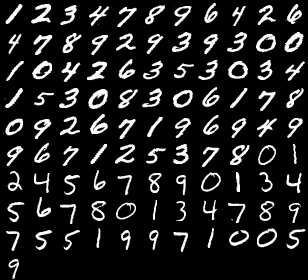
\includegraphics[width=2in]{reconstr_original.png} &
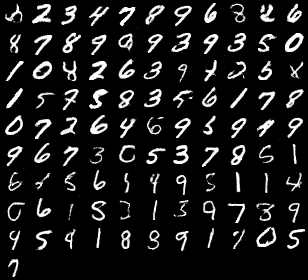
\includegraphics[width=2in]{reconstr_random_z.png} &
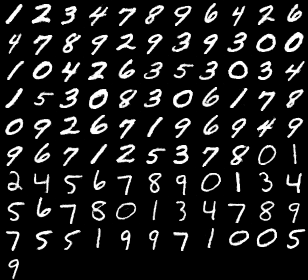
\includegraphics[width=2in]{reconstr_encoded.png} \\
random MNIST images &
$x_{proj}$ from random z &
$x_{proj}$ from $\hat{z} = \mathcal{E}_{\aplha}(x)$
\end{tabular}
\caption{Random vs. encoded initialization for random MNIST images (150 projection steps each)}

\end{figure}

As shown in figure 5, the reconstruction formed by using the initial point $\hat{z} = \mathcal{E}_{\aplha}(x) $ is visually superior; moreover, the image class is preserved with higher probability. Note that these examples are not adversarial which highlights the issue of using a random initialization. Our improved INC defence model is detailed graphically in figure 6.

\begin{figure}[H]
\centering
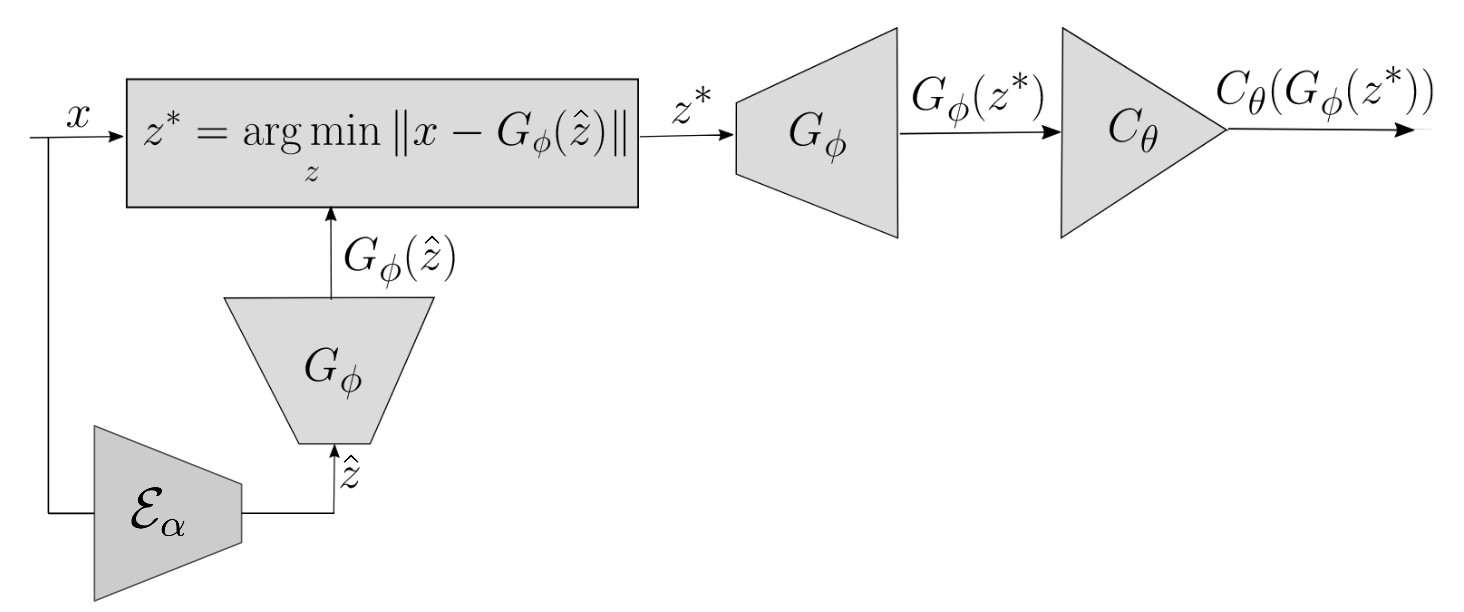
\includegraphics[scale=0.25]{INC++.png}
\caption{INC + matched encoder defense method }

\end{figure}

The below figure shows the reconstruction of adversarial images using our matched encoder as an initial point to the projection process.

%%%%%%%%%%%%%%%%%%%%%%%%%%%%%%%%%%%%%%%%%%%%%%55
% Can we show this figure in Experiment part?

\section{Critique of INC Projection}
We empirically found that using a matched encoder for initialization added robustness; moreover, it is interesting to consider why projection with random initialization is generally unstable. The two claims that follow attempt to explain why this is.

\subsection{Projection with Image Space Loss}
Looking back to the INC projection step from Problem 2, at first the formulation seems innocuous. We hope to find a $z^*$ which results in projection $x_{proj} = \mathcal{G}_{\phi}(z)$ which is close to $x_{adv}$.

\begin{equation*}
\begin{aligned}
& z^* = \text{arg } \underset{z}{\text{min}}
& & \norm{\mathcal{G}_{\phi}(z)-x_{adv}}{2}^2 \\
\end{aligned}
\end{equation*}

The problem with this formulation is that the loss is defined as an $\ell_2$ distance in the image space. Our claim is that this loss surface in the z-space is ill-conditioned with many sharp minima. For a given image class, there are a large number of candidate images (not necessarily of the same class) which produce a small $\ell_2$ loss with the true image. Assuming random initialization, we believe the INC projection is likely to fall into one of these sharp valleys and not escape.

In order to make this idea more concrete, we consider a simple example. Let us assume that our data comes from a Swiss roll distribution. Given an adversarial example $x_{adv}$ we wish to classify it (can be seen off the manifold in the figure below). We wish to find a $z$ such that $||G(z) - x_{adv}||_2$ is small. Say that the random initialization point we choose corresponds to location \emph{A} in the figure below. Using gradient descent, the projection process will encounter several ill-conditioned minima before reaching the optimal point $z^*$ which gives us the smallest reconstruction error.

\begin{figure}[H]
\begin{subfigure}{0.5\textwidth}
    \centering
    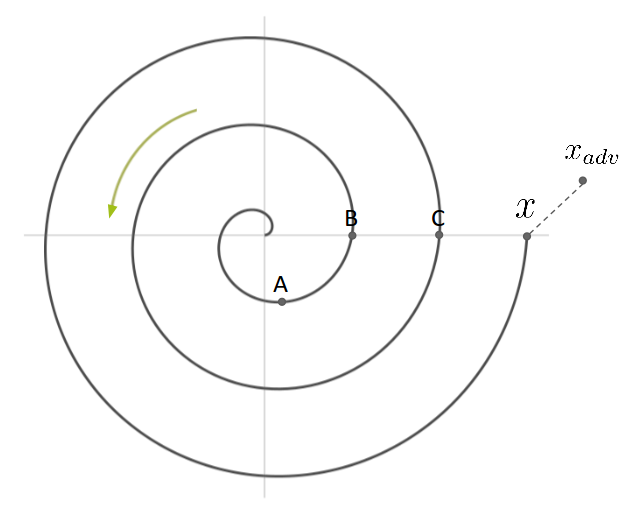
\includegraphics[scale=0.25]{./swiss.png}
    \caption{Swiss roll data in $\mathbb{R}^2$}

\end{subfigure}%
\begin{subfigure}{0.5\textwidth}  %%<--- here
    \centering
    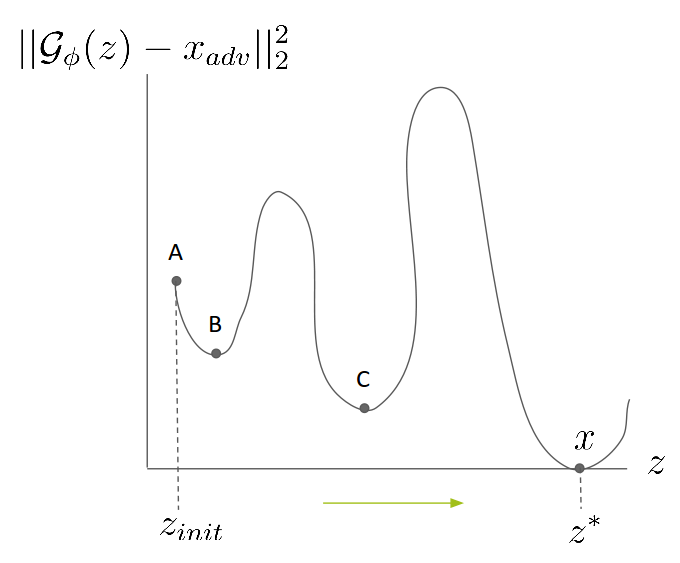
\includegraphics[scale=0.25]{./loss_swiss.png}
    \caption{Data loss vs z $\mathbb{R}^2$}
\end{subfigure}
\end{figure}

\subsection{Random Initialization}

In addition to an ill-conditioned loss surface, the INC projection step encounters another problem, now due to the random initialization. Our second claim is that for high dimensional latent spaces, the random encoding $z_{init}$, used as the starting point for optimization, is likely far from the true encoding $z$.

\begin{figure}[H]
    \centering
    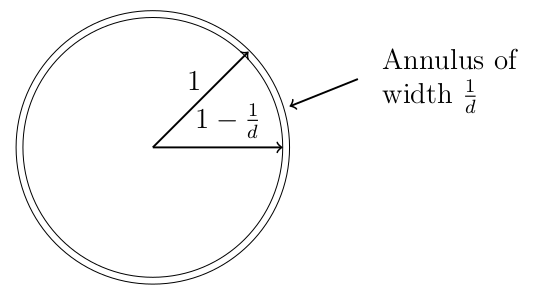
\includegraphics[scale=0.3]{./shell.png}
    \caption{Most of the probability mass is contained in a shell of width $\frac{1}{d}$ where $d$ is the dimension}
\end{figure}

For Gaussian ($N(0, 1)$) random vectors in high dimensions, $||u - v||_2^2 \approx O(d)$ \cite{foundations}, so a random initialization point in the latent space is far from the true encoding $z$ w.h.p. Accordingly, it is very likely that we will fall into a local minimum during the projection step of INC.

\begin{comment}
The true encoding $z$ and initialization $z_{init}$, both drawn from $\mathcal{N}(0,\sigma^2 \cdot I) \in \mathbb{R}^N$, are independent; thus, we can simply use the LLN to state:

$\norm{z-z_{init}}{2}^2 = \sum\limits_{i=1}^d (z_i-z_{init,i})^2 \overset{p}{\longrightarrow} d \cdot \mathbb{E}[(Z-Z_{init})^2]
= 2N \cdot \mathbb{E}[Z^2] = 2d \cdot \sigma^2$
\end{comment}


\section{Classification Experiments}

Our classification experiments were first conducted on the familiar MNIST dataset. The adversarial images $\mathcal{X}_{adv}$ were generated through FGSM attacks on the unprotected classifier $\mathcal{C}_{\theta}$. The classification accuracy results
are presented below.



\begin{center}
\begin{tabular}{ |c|c|}
 \hline
  \multicolumn{2}{|c|}{Classification Accuracy on MNIST}\\
 \hline
 Clean test data & 98\% \\ 
 \hline
 Adversarial test set using FGSM against unprotected classifier and $\epsilon = 0.2$ & 19\% \\ 
 \hline
 Adversarial test set against INC protected classifier & 87\% \\ 
 \hline
\end{tabular}
\end{center}

In addition, we perform the experiment on the Fashion-MNIST dataset and show the results below.

\begin{figure}[H]
\centering
\begin{tabular}{ccc}
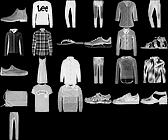
\includegraphics[width=2in]{f_mnist_original.png} &
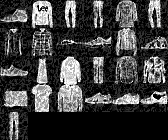
\includegraphics[width=2in]{f_mnist_adversarial.png} &
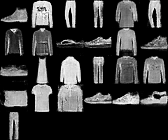
\includegraphics[width=2in]{f_mnist_reconstr_encoded.png} 
\end{tabular}
\caption{Noise level: eps = 0.2, PGD attack on Classifier with reconstructed images using our matched encoder framework}
\end{figure}

\begin{center}
\begin{tabular}{ |c|c|}
\hline
  \multicolumn{2}{|c|}{Classification Accuracy on F-MNIST}\\
 \hline
 Clean test data & 91.3\% \\ 
 \hline
 Adversarial test set using FGSM against unprotected classifier and $\epsilon = 0.2$ & 0\% \\ 
 \hline
 Adversarial test set against INC protected classifier & 60\% \\ 
 \hline
 Adversarial test set against INC with Encoder protected classifier & 69.2\%\\
 \hline
\end{tabular}
\end{center}


\section{Future Work}
The path forward from this point is to evaluate our framework on a more
complex dataset such as CelebA. This will give us a better idea of the
limitations of the matched-encoder framework. In addition, we are
interested in investigating methods for finding a better matched-encoder.

\section{Conclusion}

We have shown that using our matched-encoder framework improves the
classification accuracy on MNIST and Fashion-MNIST datasets.

If our method shows a significant improvement in classification
accuracy on CelebA, then we are confident that combining the
matched-encoder framework with the Robust Manifold Defense will yield
the best performing defense mechanism to date.

\bibliographystyle{plain}
\bibliography{ref}

\newpage

\section{Appendix}

\subsection{Direct Attack on INC}

Using our BPDA style attack on an INC protected classifier (differentiating through an encoder fitted to the generator used in the INC process) we did not arrive at the results that we had hoped for: the accuracy of the INC protected classifier remained at 93\%. Shown below are the original images, the adversarial examples created via FGSM and the images resulting from the autoencoding process.

\begin{figure}[H]
\centering
\begin{tabular}{ccc}
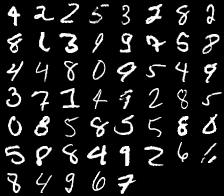
\includegraphics[width=2in]{cl_original.png} &
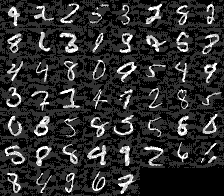
\includegraphics[width=2in]{cl_adversarial.png} &
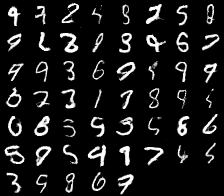
\includegraphics[width=2in]{cl_reconstr.png}
\end{tabular}
\caption{Some failure cases in MNIST test data, the adversarial examples created via FGSM and the images resulting from the autoencoding process}
\end{figure}

\end{document}